\chapter{Multi-dim Differential Calculus}

\begin{definition}[Richtungsableitung]
    Sei $\Omega \subseteq \R^n$ offen, $f:\Omega \to \R^m$ eine Funktion, $x_0 \in \Omega$ ein Punkt und $v \in \R^n$ ein Vektor. Dann bezeichnet man die \textit{Ableitung von $f$ in $x_0$ in Richtung $v$ als}
    $$ f'(x_0; v) = f'_v(x_0) =  \lim_{h \to 0} \frac{f(x_0 + hv)-f(x_0)}{h} = \frac{d}{dh} f(x_0 + hv) \bigg|_{h=0}$$
    falls dieser Grenzwert existiert. \\
    Ist $v$ normiert, also $\norm{v} =1$, dann nennt man $f'_v(x_0)$ die \textbf{Richtungsableitung} von $f$ in $x_0$ in Richtung $v$.
\end{definition}

\begin{remark}
    Spricht man von \textit{Richtungsableitung}, so muss der Richtungsvektor stets normiert werden!
\end{remark}

\section{Partielle Differenzierbarkeit}

\begin{definition}[Partielle Ableitung]
    Sei $\Omega \subset \R^n$ offen, $x_0 \in \R^n$ und unsere Funktion $f:\Omega \to \R^n$. Dann heisst \textit{$f$ an der Stelle $x_0$ partiell nach $x^i$ differenzierbar} falls der Grenzwert der Richtungsableitung in Richtung $e_i$ existiert:
    $$ \frac{\partial f}{\partial x^i}(x_0) := f_{x^i}(x_0) :=$$ $$\lim_{h\to 0} \frac{f(x_0+ h \cdot e_i)}{h} = \lim_{h\to 0} \frac{f(x_0^1, \dots, x_0^i + h, \dots, x_0^n) - f(x_0^1, \dots, x_0^n)}{h}$$
    $f$ heisst dann partiell nach $x^i$ differenzierbar in $x_0$.
\end{definition}

\begin{concept}[Partielle Ableitung berechnen]
    Gegeben sei eine Funktion $f:\R^n \to \R^m$ und gesucht sei ihre Ableitung nach $x^i$ im Punkt $x_0 \in \R^n$. Um diese zu berechnen, kann man die $f$ als 1-dimensionale Funktion auffassen, indem man alle anderen Variablen als konstant betrachtet, und dann nach $x^i$ ableiten.\\
    Besonders nützlich ist dies im Fall von Skalarfelder also $f: \R^n \to \R$.
\end{concept}

\section{Totale Differenzierbarkeit}

\begin{definition}[Totale Ableitung]
    Sei $f: \R^n \to \R^m$. Dann heisst \textit{$f$ differenzierbar an der Stelle $x_0$}, falls eine lineare Abbildung 
    $$ A: \R^n \to \R^m$$ existiert (dies ist eine $m \times n$ Matrix), so dass
    $$ \lim_{x \to x_0} \frac{|f(x) -f(x_0) - A(x-x_0)|}{|x-x_0|} = 0$$
    Dann heisst $A:= df(x_0)$ das \textit{(totale) Differential} von $f$ in $x_0$.
\end{definition}

\begin{definition}[Jacobi-Matrix]
    Das totale Differential ist eine lineare Abbildung und ist eindeutig, falls es existiert. Es ist gegeben durch die Jacobi-Matrix:
    $$ Df(x_0) = \begin{pmatrix}
    \frac{\partial f_1}{\partial x_1}(x_0)  & \dots     & \frac{\partial f_1}{\partial x_n}(x_0) \\ 
    \vdots                                  & \ddots    & \vdots \\ 
    \frac{\partial f_m}{\partial x_1}(x_0)  & \dots     & \frac{\partial f_m}{\partial x_n}(x_0)
    \end{pmatrix} $$
\end{definition}

\begin{remark}
    Um die Differenzierbarkeit einer Funktion $f$ an der Stelle $x_0$ zu überprüfen, muss man die Jacobi-Matrix an der Stelle $x_0$ berechnen und die Definition mit $u = df(x_0)$ verifizieren.
\end{remark}

\begin{theorem}
	For $f$ differentiable on $X$ we have:
	\begin{enumerate}
		\item $f$ continuous on $X$.
		\item $f$ has partial derivatives on $X$
		\item Assuming $f$ maps to $\R$, and $u(x_1,...,x_n) = a_1x_1 + ... + a_nx_n$ is its differential at $x_0 \in X$.
			Then $\partial_if(x_0) = a_i$.
	\end{enumerate}
\end{theorem}

\begin{theorem}
	If all partial derivatives for $f$ exist and are coninuous, then $f$ is differentiable.
\end{theorem}

\begin{definition}[Tangent space]
	Consider $f: X \to \R^m, \ X\subset \R^n$ open with $u=df(x_0)$.
	The affine linear approximation $g: \R^n \to \R^m,\  x \mapsto f(x_0) + u(x-x_0)$ defines the tagent space at $x_0$ to the graph of $f$.
\end{definition}

\begin{theorem}[Rechenregeln]
    Sei $\Omega\subset\R^n$ und $f,g:\Omega\to\R$ so dass $f,g$ in $x_0$ differenzierbar sind. Dann sind $f+g$, $f g$ und $f/g$ in $x_0$ differenzierbar mit:
    \begin{itemize}
        \item[(i)] $\displaystyle d(f+g)(x_0) = df(x_0) + dg(x_0)$
        \item[(ii)] $\displaystyle d(fg)(x_0) = (df)(x_0)\cdot g(x_0) + f(x_0)\cdot dg(x_0)$
        \item[(iii)] $\displaystyle d\left(\frac{f}{g}\right)(x_0) = \frac{g(x_0)\cdot df(x_0) - f(x_0)\cdot dg(x_0)}{(g(x_0))^2} \quad$ falls $g(x_0)\neq 0$
        \item If $\det(df(x_0)) \neq 0 \Rightarrow f$ is locally bijective, hence for $y = f(x)$:
			$$d(f^{-1})(y) = (df(x))^{-1} = J^{-1}_f(y)$$
			If this holds for all $x \in X$, $f$ is called a \textbf{diffeomorphism}. 
		\item For $f: X \to Y, \ g: Y \to \R^p$ differentiable, $g\circ f: X \to \R^p$ is differentiable with according to the \textbf{chain rule}:
			$$d(g\circ f)(x_0) = dg(f(x_0))\circ df(x_0), \ J_{g\circ f}(x_0) = J_g(f(x_0))J_f(x_0)$$
    \end{itemize}
\end{theorem}

\begin{theorem}
    Für eine Funktion $f: \R^n \to \R^m$ und einen Punkt $a \in \R^n$ gilt:
    \begin{center}
        $f$ ist in $a$ differenzierbar $\implies$ $f$ ist in $a$ stetig.
    \end{center}
\end{theorem}

\begin{lemma}
    Für eine Funktion $f: \R^n \to \R^m$ und einen Punkt $a \in \R^n$ gilt:
    \begin{center}
        $f$ ist in $a$ \textit{nicht} stetig $\implies$ $f$ ist in $a$ \textit{nicht} differenzierbar
    \end{center}
\end{lemma}

\section{So chli öbis}

\begin{definition}[\textbf{Klasse $C^k$}]
    $f: \Omega \subset \R^n \to \R^m$ heisst von der Klasse $C^k$, falls alle partiellen Ableitungen $k$-ter Ordnung existieren und auf $\Omega$ stetig sind.\\
    Gilt $f \in \C^k (\Omega) \; \forall k$, dann sagt man, $f$ sei von der Klasse $C^\infty(\Omega)$, d.h. $f$ ist \textit{glatt}.
\end{definition}

\begin{theorem}
    $f \in C^{k+1}(\Omega) \implies f \in C^k (\Omega)$ für alle $k \in \N_0 $.
\end{theorem}

\begin{definition}[\textbf{homogene Funktion}]
    $f: \R^n \to \R$ heisst homogen vom Grad $\lambda$, wenn für $t>0$ und alle $x \in \R^n$ gilt
    $$ f(tx) = t^\lambda f(x)$$
\end{definition}

\begin{theorem}
    $f :\R^n \to \R$ (total) differenzierbar ist homogen vom Grad $\lambda \in \R$ $$ \iff$$
    für alle $x \in \R^n$ gilt $\displaystyle \lambda f(x) = x \cdot \nabla f(x)$ wobei $\cdot$ das Skalarprodukt bezeichnet.
\end{theorem}

\section{Kettenregeln und Umkehrsatz}

\begin{theorem}[Kettenregel]
    Sei $f: \Omega \subset \R^n \to \R^m$ differenzierbar und $g: U \subset \R^m \to \R^k$ differenzierbar, wobei $U \subset f(\Omega)$. Dann ist die zusammengesetzte Abbildung $g \circ f : \Omega \subset \R^n \to \R^k$ auf $\Omega$ differenzierbar und es gilt
$$ d (g \circ f)(x) = dg(f(x)) \cdot df(x)$$
Bemerkung: Die Operation $\cdot$ bezeichnet hier eine Matrix-Multiplikation.
\end{theorem}

\begin{theorem}[Umkehrsatz]
    Ist $\det(df(x_0)) \neq 0$, so ist f lokal umkehrbar, dh es exisitieren offene Umgebungen U von $x_0$ und V von $f(x_0)$, sodass f eingeschränkt auf U $f| _U: U \to V$ bijektiv ist. Die inverse Abbildung $f| _U^{-1}: V \to U$ ist auf V von der Klasse $C^1$ und für die Ableitung gilt $$d(f^{-1})(y) = (df(x))^{-1} = \mbox{Inverse der Jacobi Matrix von f}$$ wobei $y = f(x)$
\end{theorem}

\begin{remark}
    Eine Abbildung $f: \Omega \to f(\Omega)$ heisst Diffeomorphismus, falls f invertierbar und f, $f^{-1}$ von der Klasse $C^1$ sind.Der Umkehrsatz besagt somit, dasss eine differnezierbare Abbildung mit invertierbarem Differenzial (dh $\det df \neq 0$) lokal ein Diffeomorphismus ist.
\end{remark}

\begin{concept}[Kochrezept für Diffeomorphismen]
    Gegeben: $\Phi: U \subset \R^n \to V \subset \R^n$ \\
    Gefragt: Ist $\Phi$ ein Diffeomorphismus ? \\
    \begin{itemize}
        \item Beweise, dass $\Phi$ stetig diffbar ist, berechne das Diffenrenzial $d\Phi$ (Jacobi-Matrix) und zeige, dass $\det d\Phi(x) \neq 0, \forall x \in U$
        Der Umkehrsatz impliziert, dass $\Phi$ lokal ein Diffeomorphismus ist.
        \item Beweise, dass $\Phi$ die Menge U bijektiv auf V abbildet.
    \end{itemize}
    Alternativ kann man auch die Inverse $\Phi^{-1}$ bestimmen und zeigen, dass $\Phi$ und $\Phi^{-1} \: C^1$ Funktionen sind
\end{concept}

\section{Taylorentwicklung für Funktionen mit mehreren Variablen}

\begin{definition}[\textbf{Taylor-Entwicklung}]
    Sei $f: \Omega \subset\R^n \to \R^m$ ein glattes Vektorfeld, d.h. $f \in C^\infty(\Omega)$ und $a = (a_1, \dots, a_n) \in \Omega$ ein Punkt. Dann ist die Taylor-Entwicklung von $f$ in $a$ gegeben durch
    $$ \mathit{Tf} (x; a) = \sum_{n=0}^\infty \frac{1}{n!} \left( \Delta x_1 \partial_{x_1} + \dots + \dots \Delta x_n \partial_{x_n} \right)^n f(x_1, \dots, x_n) \bigg|_{(a_1, \dots, a_n)}$$
    wobei $\Delta x_i := x_i - a_i$.
\end{definition}

\begin{remark}
    Ist $f$ ein Vektorfeld, d.h. ist $m > 1$, dann muss jede Komponente $f_i$ separat entwickelt werden.
\end{remark}

\begin{concept}[Taylor-Entwicklung für 2 Variablen bis zur 2. Ordnung]
    $$ \mathit{Tf}_2((x,y), (x_0,y_0)) =$$ $$f(x_0, y_0) + \frac{\partial f}{\partial x} \Delta x + \frac{\partial f}{\partial y} \Delta y + \frac{1}{2} \left( \frac{\partial^2 f}{\partial x^2} (\Delta x)^2 + 2 \frac{\partial^2 f}{\partial x \partial y} \Delta x \Delta y + \frac{\partial^2 f}{\partial y^2} (\Delta y)^2 \right)$$
\end{concept}

\begin{definition}[\textbf{Hesse-Matrix}]
    Sei $f:\Omega \subset \R^n \to \R$ ein zweimal differenzierbares Skalarfeld. Dann ist die \textit{Hesse-Matrix} definiert als
    $$ \mathrm{H}_f(x) = \nabla^2 f = \begin{pmatrix}
    \frac{\partial^2 f}{\partial x^1	\partial x^1} & \dots & \frac{\partial^2 f}{\partial 			x^1	\partial x^n} \\
    \vdots & \ddots & \vdots \\
    \frac{\partial^2 f}{\partial x^n	\partial x^1} & \dots & \frac{\partial^2 f}{\partial 			x^n	\partial x^n}
    \end{pmatrix}$$
    Diese Matrix ist symmetrisch, falls $f\in C^2$.
\end{definition}

\begin{theorem}[Satz von Schwarz]
    Ist $f: \Omega \to \R$ auf $\Omega$ $m$-mal partiell diff'bar und sind alle $m$-ten Ableitungen in $\Omega$ stetig, so spielt die Reihenfolge der Differantationen bei partielllen Ableitungen der Ordnung $\leq m$ keine Rolle. Daher gilt: wenn $f \in C^2(\Omega)$ ist, ist die Hessian matrix symmetrisch.
\end{theorem}

\begin{theorem}[Taylor-Entwicklung bis zur 2. Ordnung]
    $$ \mathit{Tf}(x; x_0) = f(x_0) + (x-x_0)^\top \cdot \nabla f(x_0) + \frac{1}{2} (x-x_0)^\top \cdot H_f(x_0) \cdot (x-x_0)$$
\end{theorem}

\section{Kurven}

\begin{definition}[\textbf{differenzierbare Kurve}]
    Eine \textit{differenzierbare Kurve} ist eine $C^1$-Abbildung
    $$ \gamma : [a,b] \to \R^n \quad \quad \quad t \mapsto \gamma(t)$$
    welche jedem Wert des Parameters $t$ im Intervall einen Vektor $\gamma(t) \in \R^n$ zuordnet.
    Dabei bezeichnen wir $t$ als den Parameter. Der Anfangspunkt ist gegeben durch $\gamma(a)$, der Endpunkt durch $\gamma(b)$.
\end{definition}

\begin{remark}
    Kurven können einzeln defininiert und dann zu einer Summenkurve aneinandergereiht werden.
\end{remark}

\begin{definition}[Reguläre Kurve]
    Eine diff'bare Kurve $$ \gamma: [a,b] \to \R^n, t \to \gamma(t)$$ heisst regulär, falls gilt $$\gamma'(t) = \frac{d\gamma(t)}{dt} \neq 0 \forall t \in [a,b]$$ was gleichbedeutend dazu ist, dass die Ableitungen aller Komponenten von $\gamma(t)$ nach t ungleich 0 sind.
\end{definition}

\begin{definition}[Länge einer regulären Kurve]
    Für eine reguläre Kurve $$ \gamma: [a,b] \to \R^n, t \to \gamma(t)$$ ist die Länge von $\gamma$ wie folgt zu berechnen $$L(\gamma) = \int_a^b |\gamma'(t)| dt $$
\end{definition}

\section{kritische und reguläre Punkte}
\textcolor{red}{insert stuff here}
\section{Extremwertaufgaben in mehreren Dimensionen}
\textcolor{red}{insert stuff here}

\section{Satz über implizite Funktionen}

\begin{theorem}[Implizite Funktionen]
    Sei $\Omega \subset \R^n = \R^k \times \R^l$ offen, und sei $f: \Omega \to \R^l$ stetig differenzierbar. Ist der Punkt $p_0=(a,b) \in \Omega$ regulär mit
    $$ f(p_0) = 0 \quad \quad \mbox{und} \quad \quad \det(d_yf(p_0)) \neq 0 \quad \quad \mbox{(d.h. } d_yf(p_0) \mbox{ ist invertierbar)}$$
     so lässt sich das Gleichungssystem 
    $ f(x,y) = 0 $ nach den Koordinaten $y$ auflösen. Dies bedeutet, dass eine offene Umgebung $U$ von $a$ in $\R^k$ und eine offene Umgebung $V$ von $b$ in $\R^l$ mit einem $C^1$ \textit{Diffemorphismus}\footnote{bijektive, stetig differenzierbare Abbildung, deren Umkehrfunktion ebenfalls stetig differenzierbar ist.} $h: U \to V$ existieren, so dass 
    $$ f(x, h(x)) = 0$$
    Das Differential von $h$ kann ohne explizite Funktionsvorschrift berechnet werden durch:
    $$ dh(x) = - (d_yf(x, h(x))^{-1} \cdot d_xf(x, h(x))$$
\end{theorem}

\begin{remark}
    $$ df(x,y) = \bigg(d_x f(x,y) \with d_y f(x,y) \bigg) = \begin{pmatrix}
    \frac{\partial f_1}{\partial x_1} & \cdots & \frac{\partial f_1}{\partial x_k} & 
    \frac{\partial f_1}{\partial y_1} & \cdots & \frac{\partial f_1}{\partial y_l} \\ 
    \vdots & \ddots & \vdots & \vdots & \ddots & \vdots \\
    \frac{\partial f_l}{\partial x_1} & \cdots & \frac{\partial f_l}{\partial x_k} & 
    \frac{\partial f_l}{\partial y_1} & \cdots & \frac{\partial f_l}{\partial y_l}
    \end{pmatrix} $$
    eine $l \times n$ Matrix
\end{remark}

\section{Grundbegriffe der Vektoranalysis}

\begin{remark}
    In der mehrdimensionalen Analysis unterscheidet man grundsätzlich zwei Arten von Funktionen:
    \begin{itemize}
        \item \textbf{Vektorfelder} sind Funktionen der Art $f: \R^n \to \R^m$
        \item \textbf{Skalarfelder} sind Funktionen der Art $f: \R^n \to \R$
    \end{itemize}
    Für Skalarfelder ist diese Matrix eine $1\times n$ Matrix und wird oft auch als \textbf{Gradient} bezeichnet:
    $$ \nabla f(x_0) := Df(x_0) = \begin{pmatrix}
    \frac{\partial f}{\partial x^1}(x_0) & \dots & \frac{\partial f}{\partial x^n}(x_0)
    \end{pmatrix} $$
    Dabei gibt $\nabla f(x_0)$ die Richtung und $\norm{ \nabla f(x_0)}$ die Stärke des stärksten Anstiegs in $x_0$.\\
    Für Skalarfelder kann folgendes Entscheidungsdiagramm für Differenzierbarkeit verwendet werden:
    \begin{center}
        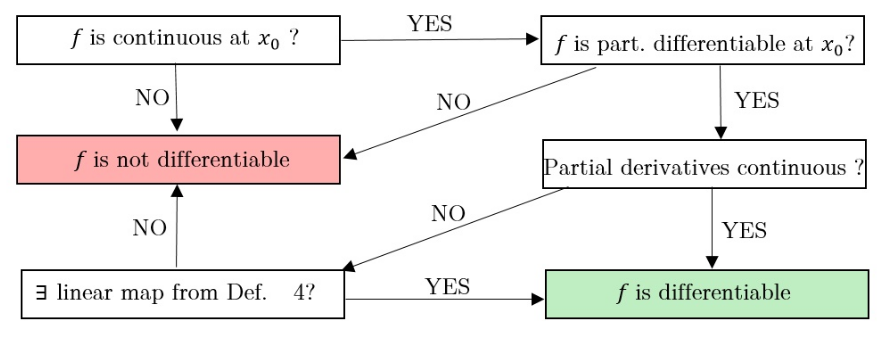
\includegraphics[scale=0.3]{img/diff.png}
    \end{center}
\end{remark}

\begin{definition}[Gradient]
	Ist $f: X \subset \R^n \to \R, $ ein stetig diff'bares Skalarfeld, so definiert man den Gradienten von f als:
	$$grad(f) = \nabla f = \begin{pmatrix} \frac{\partial f}{\partial x_1} \\ \vdots \\ \frac{\partial f}{\partial x_n} \end{pmatrix}$$
	dabei nennt man $\nabla$ den Nabla-Operator)
\end{definition}

\begin{remark}
    Die einfach partiellen Ableitungen einer Funktion kann man in einem Vektor anordnen, dem Gradienten.
    Die zweifachen partiellen Abeleitungen einer Funktion kann man in einer $n \times n$ Matrix anordnen, der Hesse-Matrix.
\end{remark}

\begin{theorem}
    Sei $f:\R^n \to \R$ ein Skalarfeld, für welches alle Richtungsableitungen in einem Punkt $a \in \R^n$ existieren. Dann existieren also auch die partiellen Ableitungen und es gilt
    $$ D_u f(a) = \nabla f(a) \cdot \frac{u}{\norm{u}} \quad \quad \forall u \in \R^n $$
\end{theorem}

\begin{definition}[Rotation]
    Für ein Vektorfeld $V: \Omega \subset \R^3 \to \R^3$ von der Klasse $C^1$ mit Komponenten $v_1, v_2, v_3$ ist die Rotation von V definiert durch 
    $$rot(V) = \begin{pmatrix} \frac{\partial v_3}{\partial y} - \frac{\partial v_2}{\partial z} \\
    \frac{\partial v_1}{\partial z} - \frac{\partial v_3}{\partial x} \\
    \frac{\partial v_2}{\partial x} - \frac{\partial v_1}{\partial y} \\
    \end{pmatrix}$$
    Die Rotation eines Vektorfelds ist also ein Vektorfeld
\end{definition}

\begin{remark}[Rotation in $\R^2$]
    $$rot(V) = \frac{\partial v_2}{\partial x} - \frac{\partial v_1}{\partial y} $$
\end{remark}

\begin{definition}[Divergenz]
    Sei $v: \Omega \subset \R^n \to \R^n$ ein Vektorfeld von der Klasse $C^1$. Dann ist die \textit{Divergenz} von $v$ definiert als 
    $$ \mathrm{div}(V) := \frac{\partial v_1}{\partial x_1} + \frac{\partial v_2}{\partial x_2} + \dots + \frac{\partial v_n}{\partial x_n},$$
    es ist also ein Skalarfeld. Eine Vektorfeld $V$ mit der Eigenschaft $\mathrm{div}(V) = 0$ nennt man quellfrei (divergenzfrei)
\end{definition}

\begin{remark}
    \textcolor{red}{Insert Ebenengleichung etc aus Serie}
\end{remark}

\begin{remark}
    Ebenengleichung in $\R^3: ax + by + cz = d $ wobei d der Abstand zum Ursprung ist \\
    
\end{remark}